% Copyright (c)  2005-2010 EDF-EADS-PHIMECA.
% Permission is granted to copy, distribute and/or modify this document
% under the terms of the GNU Free Documentation License, Version 1.2
% or any later version published by the Free Software Foundation;
% with no Invariant Sections, no Front-Cover Texts, and no Back-Cover
% Texts.  A copy of the license is included in the section entitled "GNU
% Free Documentation License".
\renewcommand{\filename}{docUC_InputWithData_EmpiricalDrawing.tex}
\renewcommand{\filetitle}{UC : Drawing Empirical CDF, Histogram, Clouds / PDF or superposition of two clouds from data}

% \HeaderNNIILevel
% \HeaderIILevel
\HeaderIIILevel



\index{Graph!Empirical cumulative density function}
\index{Graph!Histogram}
\index{Graph!Superposition two points clouds}
\index{Graph Manipulation!Bounding box}
\index{Graph Manipulation!ViewImage}
\index{Graph Manipulation!Show}



The objective of this Use Case is to draw :
\begin{itemize}
\item the empirical cumulative density function (CDF) from data : GRAPH 1,
\item the histogram from data : GRAPH 2 (with imposed number of bars) and GRAPH 3 (with free number of bars) ,
\item the superposition of two 2D samples where the first sample is given as sample and the second sample is evaluated from a given from a 2D distribution : GRAPH 4,
\item the superposition of two 2D samples where both samples are given as samples : GRAPH 5.
\end{itemize}



Details on empirical cumulative distribution function may be found in the Reference Guide (\href{OpenTURNS_ReferenceGuide.pdf}{see file Reference Guide - Step B -- Empirical cumulative distribution function}).\\

Details on each object may be found in the User Manual  (\href{OpenTURNS_UserManual_TUI.pdf}{see User Manual - Statistics on sample / Visual Test}).\\





To draw an histogram, it is possible :
\begin{itemize}
\item to fix the number of bars,
\item or not to mention it : Open TURNS will determine automatically the bandwidth of the histogram according to the Silverman rule (gaussian empirical rule).
\end{itemize}

\requirements{
  \begin{description}
  \item[$\bullet$] one scalar numerical sample : {\itshape sample}
  \item[$\bullet$] two 2D numerical samples : {\itshape sample2, sample3}
  \item[type:] NumericalSample
  \item[$\bullet$] one 2D distribution : {\itshape dist2D}
  \item[type:] Distribution
  \end{description}
}
{
  \begin{description}
  \item[$\bullet$] the files containing the empirical CDF graph : {\itshape sampleCDF.png, sampleCDF.eps, sampleCDFZoom.png, sampleCDFZoom.eps}
  \item[type:]  files at format PNG or EPS or FIG
  \item[$\bullet$] the files containing the histogram graph : {\itshape sampleHist.png, sampleHist.eps, sampleHistOpt.png, sampleHistOpt.eps}
  \item[type:]  files at format PNG or EPS or FIG
  \item[$\bullet$] the files containing the superposed samples (sample 2 and issued from dist2D)  : {\itshape sampleCloudPdf.png, sampleCloudPdf.eps}
  \item[type:]  files at format PNG or EPS or FIG
  \item[$\bullet$] the files containing the superposed samples (sample 2 and issued from dist2D)  : {\itshape sampleClouds.png, sampleClouds.eps}
  \item[type:]  files at format PNG or EPS or FIG
  \end{description}
}

\textspace\\
Python script for this UseCase :

\begin{lstlisting}
  # GRAPH 1 : Empirical CDF graph
  # Generate the Graph structure for the empirical CDF graph
  # graph range : min(sample) - 1, man(sample) + 1
  # CARE : sample must be of dimension 1
  sampleCDF = VisualTest.DrawEmpiricalCDF(sample, sample.getMin()[0] - 1.0, sample.getMax()[0] + 1.0)

  # Or impose a bounding box : x-range and y-range
  # boundingBox = [xmin, xmax, ymin, ymax]
  myBoundingBox = NumericalPoint( (xmin, xmax, ymin, ymax) )
  sampleCDF.setBoundingBox(myBoundingBox)

  # In order to see the graph without creating the associated files
  Show(sampleCDF)

  # Draw the graph on the file sampleCDF.png and sampleCDF.eps
  # if the file adress is not fulfilled, the file is created in the current directory
  sampleCDF.draw("sampleCDF")

  # View the bitmap file
  ViewImage(sampleCDF.getBitmap())

  # Check if it worked
  print "bitmap = " , sampleCDF.getBitmap()
  print "postscript = " , sampleCDF.getPostscript()

  # GRAPH 2 : Histogram graph with number of bars fixed by the user
  # Generate the Graph structure for the histogram graph
  # Number of bars fixed to 10
  # CARE : sample must be of dimension 1
  sampleHist = VisualTest.DrawHistogram(sample, 10)

  # Or zoom the histogramm : impose a bounding box : x-range and y-range
  # boundingBox = [xmin, xmax, ymin, ymax]
  myBoundingBox = NumericalPoint( (xmin, xmax, ymin, ymax) )
  sampleHist.setBoundingBox(myBoundingBox)

  # In order to see the graph without creating the associated files
  Show(sampleHist)

  # Draw the graph on the file sampleHist.png and sampleHist.eps
  # if the file adress is not fulfilled, the file is created in the current directory
  sampleHist.draw("sampleHist")

  # View the bitmap file
  ViewImage(sampleHist.getBitmap())

  # Check if it worked
  print "bitmap = " , sampleHist.getBitmap()
  print "postscript = " , sampleHist.getPostscript()

  # GRAPH 3 : Histogram graph with free number of bars
  # (automatically determined by Open TURNS according to the Silverman rule)
  # Generate the Graph structure for the histogram graph
  # CARE : sample must be of dimension 1
  sampleHistOpt = VisualTest.DrawHistogram(sample)

  # Or zoom the histogramm : impose a bounding box : x-range and y-range
  # boundingBox = [xmin, xmax, ymin, ymax]
  myBoundingBox = NumericalPoint( (xmin, xmax, ymin, ymax) )
  sampleHistOpt.setBoundingBox(myBoundingBox)

  # Draw the graph on the file sampleHistOpt.png and sampleHist.eps
  # if the file adress is not fulfilled, the file is created in the current directory
  sampleHistOpt.draw("sampleHistOpt")

  # In order to see the graph without creating the associated files
  Show(sampleHistOpt)

  # View the bitmap file
  ViewImage(sampleHistOpt.getBitmap())

  # Check if it worked
  print "bitmap = " , sampleHistOpt.getBitmap()
  print "postscript = " , sampleHistOpt.getPostscript()


  # GRAPH 4 : Superposition of two 2D samples where
  # first sample is given as sample
  # second sample is issued from a 2D distribution
  # CARE : sample2 must be of dimension 2
  # and dist is of dimension 2
  # the sample issued from dist2D have the same size than sample2
  cloudPdfGraph = VisualTest.DrawClouds(sample2, Distribution(dist2D))

  # Impose a bounding box : x-range and y-range
  # boundingBox = [xmin, xmax, ymin, ymax]
  myBoundingBox = NumericalPoint( (xmin, xmax, ymin, ymax) )
  cloudPdfGraph.setBoundingBox(myBoundingBox)

  # In order to see the graph without creating the associated files
  Show(cloudPdfGraph)

  # Draw the graph on the file sampleCloudPdf.png and sampleCloudPdf.eps
  # if the file adress is not fulfilled, the file is created in the current directory
  cloudPdfGraph.draw("sampleCloudPdf")

  # View the bitmap file
  ViewImage(cloudPdfGraph.getBitmap())

  # Check if it worked
  print "bitmap = " , cloudPdfGraph.getBitmap()
  print "postscript = " , cloudPdfGraph.getPostscript()

  # GRAPH 5 : Superposition of the two 2D samples : sample2 and sample3
  # CARE : sample2 and sample3 must be of dimension 2
  cloudPdfGraph2 = VisualTest.DrawClouds(sample2, sample3)

  # Impose a bounding box : x-range and y-range
  # boundingBox = [xmin, xmax, ymin, ymax]
  myBoundingBox = NumericalPoint( (xmin, xmax, ymin, ymax) )
  cloudPdfGraph.setBoundingBox(myBoundingBox)

  # In order to see the graph without creating the associated files
  Show(cloudPdfGraph2)

  # Draw the graph on the file sampleCloudPdf.png and sampleCloudPdf.eps
  # if the file adress is not fulfilled, the file is created in the current directory
  cloudPdfGraph2.draw("sampleClouds")

  # View the bitmap file
  ViewImage(cloudPdfGraph2.getBitmap())

  # Check if it worked
  print "bitmap = " , cloudPdfGraph2.getBitmap()
  print "postscript = " , cloudPdfGraph2.getPostscript()
\end{lstlisting}
\textspace\\



For example, Figure \ref{HistogramData} contains the  GRAPH3 obtained with a sample of size 1000 from a Normal(0.0, 1.0) distribution.\\

For example, Figure \ref{superpositionTwoclouds} contains the GRAPH4 obtained by giving :
\begin{itemize}
\item a sample (actually generated from a 2D Normal distribution with (2.0, 2.0) mean (1.0, 1.0) standard deviation and $\rho = -0.8$ correlation coefficient),
\item a 2D Normal distribution with (2.0, 2.0) mean (1.0, 1.0) standard deviation and $\rho = +0.8$ correlation coefficient
\end{itemize}


\begin{figure}[H]
  \begin{minipage}{9.8cm}
    \begin{center}
      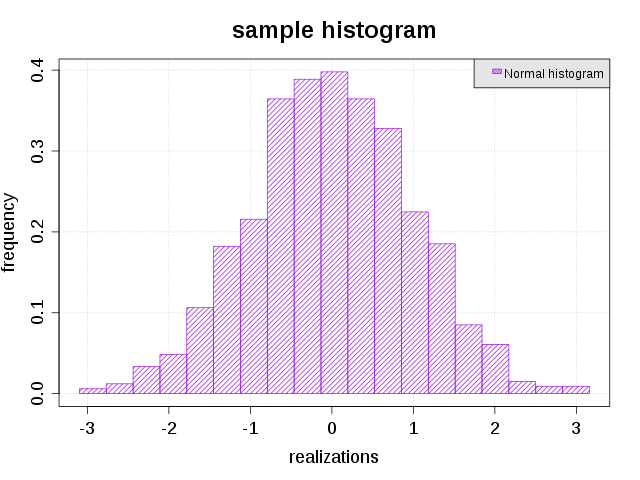
\includegraphics[width=7cm]{hist_Data.png}
      \caption{Histogram from a sample.}
      \label{HistogramData}
    \end{center}
  \end{minipage}
  \hfill
  \begin{minipage}{9.8cm}
    \begin{center}
      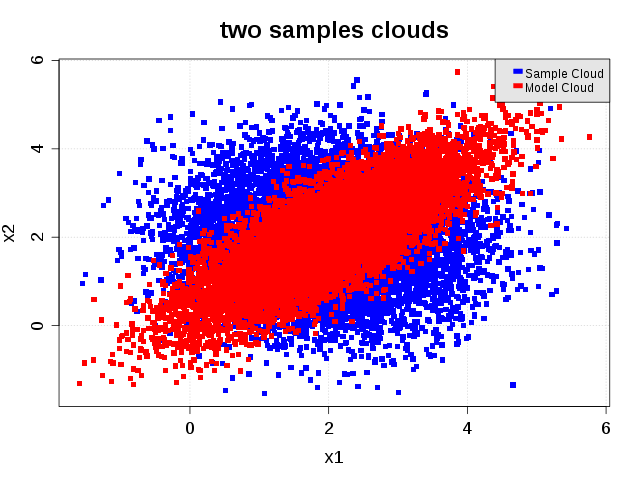
\includegraphics[width=7cm]{cloud1.png}
      \caption{Superposition of two 2D clouds.}
      \label{superpositionTwoclouds}
    \end{center}
  \end{minipage}
\end{figure}


